\documentclass[11pt]{article}
\usepackage[T1]{fontenc}
\usepackage[utf8]{inputenc}
\usepackage{lmodern}
\usepackage[margin=1in]{geometry}
\usepackage{amsmath,amssymb,amsthm}
\usepackage{booktabs}
\usepackage{graphicx}
\usepackage{xcolor}
\usepackage{microtype}
\usepackage[numbers,sort&compress]{natbib}
\usepackage[hidelinks]{hyperref}
\usepackage{tikz}
\usetikzlibrary{positioning,decorations.pathreplacing}

\newtheorem{theorem}{Theorem}
\newtheorem{lemma}[theorem]{Lemma}
\theoremstyle{definition}
\newtheorem{definition}[theorem]{Definition}

% Generated by benchmarks/scripts/bucketization_paper_numbers.py. Do not edit.
\makeatletter
\expandafter\def\csname bz@syn@linux@10000@name@std_sort_ms\endcsname{1.7}
\expandafter\def\csname bz@syn@linux@10000@name@presort_ms\endcsname{1.7}
\expandafter\def\csname bz@syn@linux@10000@name@switch_first_page_ms\endcsname{0.025}
\expandafter\def\csname bz@syn@linux@10000@name@cached_switch_ms\endcsname{0.0003}
\expandafter\def\csname bz@syn@linux@10000@name@switch_sort_all_ms\endcsname{1.0}
\expandafter\def\csname bz@syn@linux@10000@name@speedup\endcsname{69}
\expandafter\def\csname bz@syn@linux@10000@size@std_sort_ms\endcsname{0.96}
\expandafter\def\csname bz@syn@linux@10000@size@presort_ms\endcsname{1.6}
\expandafter\def\csname bz@syn@linux@10000@size@switch_first_page_ms\endcsname{0.016}
\expandafter\def\csname bz@syn@linux@10000@size@cached_switch_ms\endcsname{0.0003}
\expandafter\def\csname bz@syn@linux@10000@size@switch_sort_all_ms\endcsname{0.58}
\expandafter\def\csname bz@syn@linux@10000@size@speedup\endcsname{61}
\expandafter\def\csname bz@syn@linux@10000@modified@std_sort_ms\endcsname{0.92}
\expandafter\def\csname bz@syn@linux@10000@modified@presort_ms\endcsname{1.6}
\expandafter\def\csname bz@syn@linux@10000@modified@switch_first_page_ms\endcsname{0.016}
\expandafter\def\csname bz@syn@linux@10000@modified@cached_switch_ms\endcsname{0.0003}
\expandafter\def\csname bz@syn@linux@10000@modified@switch_sort_all_ms\endcsname{0.48}
\expandafter\def\csname bz@syn@linux@10000@modified@speedup\endcsname{59}
\expandafter\def\csname bz@syn@linux@10000@accessed@std_sort_ms\endcsname{0.96}
\expandafter\def\csname bz@syn@linux@10000@accessed@presort_ms\endcsname{1.7}
\expandafter\def\csname bz@syn@linux@10000@accessed@switch_first_page_ms\endcsname{0.013}
\expandafter\def\csname bz@syn@linux@10000@accessed@cached_switch_ms\endcsname{0.0003}
\expandafter\def\csname bz@syn@linux@10000@accessed@switch_sort_all_ms\endcsname{0.54}
\expandafter\def\csname bz@syn@linux@10000@accessed@speedup\endcsname{72}
\expandafter\def\csname bz@syn@linux@100000@name@std_sort_ms\endcsname{41}
\expandafter\def\csname bz@syn@linux@100000@name@presort_ms\endcsname{13}
\expandafter\def\csname bz@syn@linux@100000@name@switch_first_page_ms\endcsname{0.18}
\expandafter\def\csname bz@syn@linux@100000@name@cached_switch_ms\endcsname{0.0010}
\expandafter\def\csname bz@syn@linux@100000@name@switch_sort_all_ms\endcsname{41}
\expandafter\def\csname bz@syn@linux@100000@name@speedup\endcsname{226}
\expandafter\def\csname bz@syn@linux@100000@size@std_sort_ms\endcsname{22}
\expandafter\def\csname bz@syn@linux@100000@size@presort_ms\endcsname{14}
\expandafter\def\csname bz@syn@linux@100000@size@switch_first_page_ms\endcsname{0.16}
\expandafter\def\csname bz@syn@linux@100000@size@cached_switch_ms\endcsname{0.0014}
\expandafter\def\csname bz@syn@linux@100000@size@switch_sort_all_ms\endcsname{10}
\expandafter\def\csname bz@syn@linux@100000@size@speedup\endcsname{138}
\expandafter\def\csname bz@syn@linux@100000@modified@std_sort_ms\endcsname{18}
\expandafter\def\csname bz@syn@linux@100000@modified@presort_ms\endcsname{13}
\expandafter\def\csname bz@syn@linux@100000@modified@switch_first_page_ms\endcsname{0.13}
\expandafter\def\csname bz@syn@linux@100000@modified@cached_switch_ms\endcsname{0.0009}
\expandafter\def\csname bz@syn@linux@100000@modified@switch_sort_all_ms\endcsname{8.0}
\expandafter\def\csname bz@syn@linux@100000@modified@speedup\endcsname{140}
\expandafter\def\csname bz@syn@linux@100000@accessed@std_sort_ms\endcsname{20}
\expandafter\def\csname bz@syn@linux@100000@accessed@presort_ms\endcsname{15}
\expandafter\def\csname bz@syn@linux@100000@accessed@switch_first_page_ms\endcsname{0.15}
\expandafter\def\csname bz@syn@linux@100000@accessed@cached_switch_ms\endcsname{0.0010}
\expandafter\def\csname bz@syn@linux@100000@accessed@switch_sort_all_ms\endcsname{8.9}
\expandafter\def\csname bz@syn@linux@100000@accessed@speedup\endcsname{133}
\expandafter\def\csname bz@syn@linux@1000000@name@std_sort_ms\endcsname{1{,}052}
\expandafter\def\csname bz@syn@linux@1000000@name@presort_ms\endcsname{135}
\expandafter\def\csname bz@syn@linux@1000000@name@switch_first_page_ms\endcsname{2.1}
\expandafter\def\csname bz@syn@linux@1000000@name@cached_switch_ms\endcsname{0.0045}
\expandafter\def\csname bz@syn@linux@1000000@name@switch_sort_all_ms\endcsname{781}
\expandafter\def\csname bz@syn@linux@1000000@name@speedup\endcsname{501}
\expandafter\def\csname bz@syn@linux@1000000@size@std_sort_ms\endcsname{416}
\expandafter\def\csname bz@syn@linux@1000000@size@presort_ms\endcsname{130}
\expandafter\def\csname bz@syn@linux@1000000@size@switch_first_page_ms\endcsname{1.8}
\expandafter\def\csname bz@syn@linux@1000000@size@cached_switch_ms\endcsname{0.0049}
\expandafter\def\csname bz@syn@linux@1000000@size@switch_sort_all_ms\endcsname{145}
\expandafter\def\csname bz@syn@linux@1000000@size@speedup\endcsname{235}
\expandafter\def\csname bz@syn@linux@1000000@modified@std_sort_ms\endcsname{448}
\expandafter\def\csname bz@syn@linux@1000000@modified@presort_ms\endcsname{137}
\expandafter\def\csname bz@syn@linux@1000000@modified@switch_first_page_ms\endcsname{2.1}
\expandafter\def\csname bz@syn@linux@1000000@modified@cached_switch_ms\endcsname{0.0048}
\expandafter\def\csname bz@syn@linux@1000000@modified@switch_sort_all_ms\endcsname{151}
\expandafter\def\csname bz@syn@linux@1000000@modified@speedup\endcsname{212}
\expandafter\def\csname bz@syn@linux@1000000@accessed@std_sort_ms\endcsname{433}
\expandafter\def\csname bz@syn@linux@1000000@accessed@presort_ms\endcsname{119}
\expandafter\def\csname bz@syn@linux@1000000@accessed@switch_first_page_ms\endcsname{1.8}
\expandafter\def\csname bz@syn@linux@1000000@accessed@cached_switch_ms\endcsname{0.0050}
\expandafter\def\csname bz@syn@linux@1000000@accessed@switch_sort_all_ms\endcsname{131}
\expandafter\def\csname bz@syn@linux@1000000@accessed@speedup\endcsname{238}
\expandafter\def\csname bz@syn@windows@10000@name@std_sort_ms\endcsname{2.1}
\expandafter\def\csname bz@syn@windows@10000@name@presort_ms\endcsname{2.1}
\expandafter\def\csname bz@syn@windows@10000@name@switch_first_page_ms\endcsname{0.037}
\expandafter\def\csname bz@syn@windows@10000@name@cached_switch_ms\endcsname{0.0006}
\expandafter\def\csname bz@syn@windows@10000@name@switch_sort_all_ms\endcsname{1.2}
\expandafter\def\csname bz@syn@windows@10000@name@speedup\endcsname{56}
\expandafter\def\csname bz@syn@windows@10000@size@std_sort_ms\endcsname{1.1}
\expandafter\def\csname bz@syn@windows@10000@size@presort_ms\endcsname{2.3}
\expandafter\def\csname bz@syn@windows@10000@size@switch_first_page_ms\endcsname{0.029}
\expandafter\def\csname bz@syn@windows@10000@size@cached_switch_ms\endcsname{0.0006}
\expandafter\def\csname bz@syn@windows@10000@size@switch_sort_all_ms\endcsname{0.61}
\expandafter\def\csname bz@syn@windows@10000@size@speedup\endcsname{40}
\expandafter\def\csname bz@syn@windows@10000@modified@std_sort_ms\endcsname{1.1}
\expandafter\def\csname bz@syn@windows@10000@modified@presort_ms\endcsname{1.9}
\expandafter\def\csname bz@syn@windows@10000@modified@switch_first_page_ms\endcsname{0.025}
\expandafter\def\csname bz@syn@windows@10000@modified@cached_switch_ms\endcsname{0.0005}
\expandafter\def\csname bz@syn@windows@10000@modified@switch_sort_all_ms\endcsname{0.56}
\expandafter\def\csname bz@syn@windows@10000@modified@speedup\endcsname{43}
\expandafter\def\csname bz@syn@windows@10000@accessed@std_sort_ms\endcsname{1.1}
\expandafter\def\csname bz@syn@windows@10000@accessed@presort_ms\endcsname{2.0}
\expandafter\def\csname bz@syn@windows@10000@accessed@switch_first_page_ms\endcsname{0.031}
\expandafter\def\csname bz@syn@windows@10000@accessed@cached_switch_ms\endcsname{0.0005}
\expandafter\def\csname bz@syn@windows@10000@accessed@switch_sort_all_ms\endcsname{0.57}
\expandafter\def\csname bz@syn@windows@10000@accessed@speedup\endcsname{35}
\expandafter\def\csname bz@syn@windows@100000@name@std_sort_ms\endcsname{48}
\expandafter\def\csname bz@syn@windows@100000@name@presort_ms\endcsname{16}
\expandafter\def\csname bz@syn@windows@100000@name@switch_first_page_ms\endcsname{0.30}
\expandafter\def\csname bz@syn@windows@100000@name@cached_switch_ms\endcsname{0.0006}
\expandafter\def\csname bz@syn@windows@100000@name@switch_sort_all_ms\endcsname{33}
\expandafter\def\csname bz@syn@windows@100000@name@speedup\endcsname{161}
\expandafter\def\csname bz@syn@windows@100000@size@std_sort_ms\endcsname{26}
\expandafter\def\csname bz@syn@windows@100000@size@presort_ms\endcsname{17}
\expandafter\def\csname bz@syn@windows@100000@size@switch_first_page_ms\endcsname{0.25}
\expandafter\def\csname bz@syn@windows@100000@size@cached_switch_ms\endcsname{0.0007}
\expandafter\def\csname bz@syn@windows@100000@size@switch_sort_all_ms\endcsname{10}
\expandafter\def\csname bz@syn@windows@100000@size@speedup\endcsname{105}
\expandafter\def\csname bz@syn@windows@100000@modified@std_sort_ms\endcsname{24}
\expandafter\def\csname bz@syn@windows@100000@modified@presort_ms\endcsname{17}
\expandafter\def\csname bz@syn@windows@100000@modified@switch_first_page_ms\endcsname{0.26}
\expandafter\def\csname bz@syn@windows@100000@modified@cached_switch_ms\endcsname{0.0007}
\expandafter\def\csname bz@syn@windows@100000@modified@switch_sort_all_ms\endcsname{11}
\expandafter\def\csname bz@syn@windows@100000@modified@speedup\endcsname{92}
\expandafter\def\csname bz@syn@windows@100000@accessed@std_sort_ms\endcsname{40}
\expandafter\def\csname bz@syn@windows@100000@accessed@presort_ms\endcsname{24}
\expandafter\def\csname bz@syn@windows@100000@accessed@switch_first_page_ms\endcsname{0.29}
\expandafter\def\csname bz@syn@windows@100000@accessed@cached_switch_ms\endcsname{0.0008}
\expandafter\def\csname bz@syn@windows@100000@accessed@switch_sort_all_ms\endcsname{13}
\expandafter\def\csname bz@syn@windows@100000@accessed@speedup\endcsname{136}
\expandafter\def\csname bz@syn@windows@1000000@name@std_sort_ms\endcsname{1{,}088}
\expandafter\def\csname bz@syn@windows@1000000@name@presort_ms\endcsname{152}
\expandafter\def\csname bz@syn@windows@1000000@name@switch_first_page_ms\endcsname{4.5}
\expandafter\def\csname bz@syn@windows@1000000@name@cached_switch_ms\endcsname{0.0038}
\expandafter\def\csname bz@syn@windows@1000000@name@switch_sort_all_ms\endcsname{1{,}214}
\expandafter\def\csname bz@syn@windows@1000000@name@speedup\endcsname{243}
\expandafter\def\csname bz@syn@windows@1000000@size@std_sort_ms\endcsname{363}
\expandafter\def\csname bz@syn@windows@1000000@size@presort_ms\endcsname{138}
\expandafter\def\csname bz@syn@windows@1000000@size@switch_first_page_ms\endcsname{4.3}
\expandafter\def\csname bz@syn@windows@1000000@size@cached_switch_ms\endcsname{0.0048}
\expandafter\def\csname bz@syn@windows@1000000@size@switch_sort_all_ms\endcsname{135}
\expandafter\def\csname bz@syn@windows@1000000@size@speedup\endcsname{85}
\expandafter\def\csname bz@syn@windows@1000000@modified@std_sort_ms\endcsname{419}
\expandafter\def\csname bz@syn@windows@1000000@modified@presort_ms\endcsname{137}
\expandafter\def\csname bz@syn@windows@1000000@modified@switch_first_page_ms\endcsname{4.0}
\expandafter\def\csname bz@syn@windows@1000000@modified@cached_switch_ms\endcsname{0.0050}
\expandafter\def\csname bz@syn@windows@1000000@modified@switch_sort_all_ms\endcsname{147}
\expandafter\def\csname bz@syn@windows@1000000@modified@speedup\endcsname{104}
\expandafter\def\csname bz@syn@windows@1000000@accessed@std_sort_ms\endcsname{358}
\expandafter\def\csname bz@syn@windows@1000000@accessed@presort_ms\endcsname{139}
\expandafter\def\csname bz@syn@windows@1000000@accessed@switch_first_page_ms\endcsname{4.5}
\expandafter\def\csname bz@syn@windows@1000000@accessed@cached_switch_ms\endcsname{0.0047}
\expandafter\def\csname bz@syn@windows@1000000@accessed@switch_sort_all_ms\endcsname{128}
\expandafter\def\csname bz@syn@windows@1000000@accessed@speedup\endcsname{79}
\expandafter\def\csname bz@sum@linux@dolphin@resort\endcsname{59--713}
\expandafter\def\csname bz@sum@linux@dolphin@switch\endcsname{0.080--0.72}
\expandafter\def\csname bz@sum@linux@dolphin@speedup\endcsname{178--3{,}842}
\expandafter\def\csname bz@sum@linux@dolphin@presort\endcsname{2.1--73}
\expandafter\def\csname bz@sum@linux@dolphin@valid\endcsname{54/54}
\expandafter\def\csname bz@sum@linux@dolphin@invalid\endcsname{0}
\expandafter\def\csname bz@sum@linux@dolphin@slower\endcsname{0}
\expandafter\def\csname bz@sum@linux@thunar@resort\endcsname{38--333}
\expandafter\def\csname bz@sum@linux@thunar@switch\endcsname{0.047--0.30}
\expandafter\def\csname bz@sum@linux@thunar@speedup\endcsname{218--1{,}552}
\expandafter\def\csname bz@sum@linux@thunar@presort\endcsname{2.8--10}
\expandafter\def\csname bz@sum@linux@thunar@valid\endcsname{42/42}
\expandafter\def\csname bz@sum@linux@thunar@invalid\endcsname{0}
\expandafter\def\csname bz@sum@linux@thunar@slower\endcsname{0}
\expandafter\def\csname bz@sum@linux@nemo@resort\endcsname{36--382}
\expandafter\def\csname bz@sum@linux@nemo@switch\endcsname{0.057--0.22}
\expandafter\def\csname bz@sum@linux@nemo@speedup\endcsname{380--2{,}206}
\expandafter\def\csname bz@sum@linux@nemo@presort\endcsname{2.6--11}
\expandafter\def\csname bz@sum@linux@nemo@valid\endcsname{42/42}
\expandafter\def\csname bz@sum@linux@nemo@invalid\endcsname{0}
\expandafter\def\csname bz@sum@linux@nemo@slower\endcsname{0}
\expandafter\def\csname bz@sum@linux@caja@resort\endcsname{45--389}
\expandafter\def\csname bz@sum@linux@caja@switch\endcsname{0.048--0.24}
\expandafter\def\csname bz@sum@linux@caja@speedup\endcsname{312--1{,}953}
\expandafter\def\csname bz@sum@linux@caja@presort\endcsname{2.5--10}
\expandafter\def\csname bz@sum@linux@caja@valid\endcsname{42/42}
\expandafter\def\csname bz@sum@linux@caja@invalid\endcsname{0}
\expandafter\def\csname bz@sum@linux@caja@slower\endcsname{0}
\expandafter\def\csname bz@sum@linux@nautilus@resort\endcsname{63--480}
\expandafter\def\csname bz@sum@linux@nautilus@switch\endcsname{0.052--0.26}
\expandafter\def\csname bz@sum@linux@nautilus@speedup\endcsname{729--2{,}921}
\expandafter\def\csname bz@sum@linux@nautilus@presort\endcsname{2.6--12}
\expandafter\def\csname bz@sum@linux@nautilus@valid\endcsname{42/42}
\expandafter\def\csname bz@sum@linux@nautilus@invalid\endcsname{0}
\expandafter\def\csname bz@sum@linux@nautilus@slower\endcsname{0}
\expandafter\def\csname bz@sum@linux@pcmanfm-qt@resort\endcsname{48--1{,}499}
\expandafter\def\csname bz@sum@linux@pcmanfm-qt@switch\endcsname{0.092--2.0}
\expandafter\def\csname bz@sum@linux@pcmanfm-qt@speedup\endcsname{322--7{,}640}
\expandafter\def\csname bz@sum@linux@pcmanfm-qt@presort\endcsname{2.6--206}
\expandafter\def\csname bz@sum@linux@pcmanfm-qt@valid\endcsname{42/42}
\expandafter\def\csname bz@sum@linux@pcmanfm-qt@invalid\endcsname{0}
\expandafter\def\csname bz@sum@linux@pcmanfm-qt@slower\endcsname{0}
\expandafter\def\csname bz@sum@linux@kio@resort\endcsname{84--1{,}384}
\expandafter\def\csname bz@sum@linux@kio@switch\endcsname{0.079--1.2}
\expandafter\def\csname bz@sum@linux@kio@speedup\endcsname{356--6{,}647}
\expandafter\def\csname bz@sum@linux@kio@presort\endcsname{2.0--159}
\expandafter\def\csname bz@sum@linux@kio@valid\endcsname{42/42}
\expandafter\def\csname bz@sum@linux@kio@invalid\endcsname{0}
\expandafter\def\csname bz@sum@linux@kio@slower\endcsname{0}
\expandafter\def\csname bz@sum@linux@krusader@resort\endcsname{115--801}
\expandafter\def\csname bz@sum@linux@krusader@switch\endcsname{0.056--0.54}
\expandafter\def\csname bz@sum@linux@krusader@speedup\endcsname{587--4{,}207}
\expandafter\def\csname bz@sum@linux@krusader@presort\endcsname{1.9--68}
\expandafter\def\csname bz@sum@linux@krusader@valid\endcsname{42/42}
\expandafter\def\csname bz@sum@linux@krusader@invalid\endcsname{0}
\expandafter\def\csname bz@sum@linux@krusader@slower\endcsname{0}
\expandafter\def\csname bz@sum@linux@nnn@resort\endcsname{7.7--290}
\expandafter\def\csname bz@sum@linux@nnn@switch\endcsname{0.072--0.28}
\expandafter\def\csname bz@sum@linux@nnn@speedup\endcsname{72--1{,}379}
\expandafter\def\csname bz@sum@linux@nnn@presort\endcsname{1.9--106}
\expandafter\def\csname bz@sum@linux@nnn@valid\endcsname{42/42}
\expandafter\def\csname bz@sum@linux@nnn@invalid\endcsname{0}
\expandafter\def\csname bz@sum@linux@nnn@slower\endcsname{0}
\expandafter\def\csname bz@sum@linux@yazinative@resort\endcsname{6.3--63}
\expandafter\def\csname bz@sum@linux@yazinative@switch\endcsname{0.060--0.33}
\expandafter\def\csname bz@sum@linux@yazinative@speedup\endcsname{37--425}
\expandafter\def\csname bz@sum@linux@yazinative@presort\endcsname{1.5--12}
\expandafter\def\csname bz@sum@linux@yazinative@valid\endcsname{42/42}
\expandafter\def\csname bz@sum@linux@yazinative@invalid\endcsname{0}
\expandafter\def\csname bz@sum@linux@yazinative@slower\endcsname{0}
\expandafter\def\csname bz@sum@linux@lfnative@resort\endcsname{8.0--3{,}050}
\expandafter\def\csname bz@sum@linux@lfnative@switch\endcsname{0.057--1.0}
\expandafter\def\csname bz@sum@linux@lfnative@speedup\endcsname{8.3--12{,}108}
\expandafter\def\csname bz@sum@linux@lfnative@presort\endcsname{1.3--184}
\expandafter\def\csname bz@sum@linux@lfnative@valid\endcsname{42/42}
\expandafter\def\csname bz@sum@linux@lfnative@invalid\endcsname{0}
\expandafter\def\csname bz@sum@linux@lfnative@slower\endcsname{0}
\expandafter\def\csname bz@sum@linux@godot@resort\endcsname{4.3--1{,}165}
\expandafter\def\csname bz@sum@linux@godot@switch\endcsname{0.089--3.0}
\expandafter\def\csname bz@sum@linux@godot@speedup\endcsname{13--871}
\expandafter\def\csname bz@sum@linux@godot@presort\endcsname{1.2--1{,}261}
\expandafter\def\csname bz@sum@linux@godot@valid\endcsname{36/36}
\expandafter\def\csname bz@sum@linux@godot@invalid\endcsname{0}
\expandafter\def\csname bz@sum@linux@godot@slower\endcsname{6}
\expandafter\def\csname bz@sum@linux@all@speedup\endcsname{8.3--12{,}108}
\expandafter\def\csname bz@sum@linux@all@speedupmedian\endcsname{826}
\expandafter\def\csname bz@sum@linux@all@switch\endcsname{0.047--3.0}
\expandafter\def\csname bz@sum@linux@all@resort\endcsname{4.3--3{,}050}
\expandafter\def\csname bz@sum@linux@all@presortmedian\endcsname{7.0}
\expandafter\def\csname bz@sum@linux@all@valid\endcsname{510}
\expandafter\def\csname bz@sum@linux@all@total\endcsname{510}
\expandafter\def\csname bz@sum@linux@all@slower\endcsname{6}
\expandafter\def\csname bz@sum@linux@all@cases\endcsname{288}
\expandafter\def\csname bz@sum@windows@nnn@resort\endcsname{36--2{,}257}
\expandafter\def\csname bz@sum@windows@nnn@switch\endcsname{0.14--0.69}
\expandafter\def\csname bz@sum@windows@nnn@speedup\endcsname{145--4{,}639}
\expandafter\def\csname bz@sum@windows@nnn@presort\endcsname{2.6--285}
\expandafter\def\csname bz@sum@windows@nnn@valid\endcsname{32/42}
\expandafter\def\csname bz@sum@windows@nnn@invalid\endcsname{10}
\expandafter\def\csname bz@sum@windows@nnn@slower\endcsname{0}
\expandafter\def\csname bz@sum@windows@yazinative@resort\endcsname{7.7--67}
\expandafter\def\csname bz@sum@windows@yazinative@switch\endcsname{0.089--0.43}
\expandafter\def\csname bz@sum@windows@yazinative@speedup\endcsname{40--286}
\expandafter\def\csname bz@sum@windows@yazinative@presort\endcsname{1.3--16}
\expandafter\def\csname bz@sum@windows@yazinative@valid\endcsname{42/42}
\expandafter\def\csname bz@sum@windows@yazinative@invalid\endcsname{0}
\expandafter\def\csname bz@sum@windows@yazinative@slower\endcsname{0}
\expandafter\def\csname bz@sum@windows@lf@resort\endcsname{4.0--1{,}904}
\expandafter\def\csname bz@sum@windows@lf@switch\endcsname{0.080--1.2}
\expandafter\def\csname bz@sum@windows@lf@speedup\endcsname{8.8--6{,}503}
\expandafter\def\csname bz@sum@windows@lf@presort\endcsname{1.1--336}
\expandafter\def\csname bz@sum@windows@lf@valid\endcsname{42/42}
\expandafter\def\csname bz@sum@windows@lf@invalid\endcsname{0}
\expandafter\def\csname bz@sum@windows@lf@slower\endcsname{0}
\expandafter\def\csname bz@sum@windows@godot@resort\endcsname{3.6--2{,}391}
\expandafter\def\csname bz@sum@windows@godot@switch\endcsname{0.13--6.4}
\expandafter\def\csname bz@sum@windows@godot@speedup\endcsname{5.2--879}
\expandafter\def\csname bz@sum@windows@godot@presort\endcsname{1.6--2{,}510}
\expandafter\def\csname bz@sum@windows@godot@valid\endcsname{36/36}
\expandafter\def\csname bz@sum@windows@godot@invalid\endcsname{0}
\expandafter\def\csname bz@sum@windows@godot@slower\endcsname{8}
\expandafter\def\csname bz@sum@windows@all@speedup\endcsname{5.2--6{,}503}
\expandafter\def\csname bz@sum@windows@all@speedupmedian\endcsname{148}
\expandafter\def\csname bz@sum@windows@all@switch\endcsname{0.080--6.4}
\expandafter\def\csname bz@sum@windows@all@resort\endcsname{3.6--2{,}391}
\expandafter\def\csname bz@sum@windows@all@presortmedian\endcsname{9.7}
\expandafter\def\csname bz@sum@windows@all@valid\endcsname{152}
\expandafter\def\csname bz@sum@windows@all@total\endcsname{162}
\expandafter\def\csname bz@sum@windows@all@slower\endcsname{8}
\expandafter\def\csname bz@sum@windows@all@cases\endcsname{90}
\expandafter\def\csname bz@dol@partial@median\endcsname{9.1}
\expandafter\def\csname bz@dol@partial@range\endcsname{2.9--849}
\expandafter\def\csname bz@dol@partial@worst\endcsname{212}
\expandafter\def\csname bz@dol@cmp@presortratio\endcsname{0.7--3.2}
\expandafter\def\csname bz@dol@usr-bin@name@asc@resort\endcsname{3.1}
\expandafter\def\csname bz@dol@usr-bin@name@asc@switch\endcsname{0.0034}
\expandafter\def\csname bz@dol@usr-bin@name@asc@partial\endcsname{0.38}
\expandafter\def\csname bz@dol@usr-bin@name@asc@presort\endcsname{0.36}
\expandafter\def\csname bz@dol@usr-bin@name@asc@fpc\endcsname{65}
\expandafter\def\csname bz@dol@usr-bin@name@desc@resort\endcsname{3.4}
\expandafter\def\csname bz@dol@usr-bin@name@desc@switch\endcsname{0.018}
\expandafter\def\csname bz@dol@usr-bin@name@desc@partial\endcsname{0.32}
\expandafter\def\csname bz@dol@usr-bin@name@desc@presort\endcsname{0.36}
\expandafter\def\csname bz@dol@usr-bin@name@desc@fpc\endcsname{65}
\expandafter\def\csname bz@dol@usr-bin@size@asc@resort\endcsname{0.52}
\expandafter\def\csname bz@dol@usr-bin@size@asc@switch\endcsname{0.0057}
\expandafter\def\csname bz@dol@usr-bin@size@asc@partial\endcsname{0.017}
\expandafter\def\csname bz@dol@usr-bin@size@asc@presort\endcsname{0.20}
\expandafter\def\csname bz@dol@usr-bin@size@asc@fpc\endcsname{65}
\expandafter\def\csname bz@dol@usr-bin@size@desc@resort\endcsname{0.51}
\expandafter\def\csname bz@dol@usr-bin@size@desc@switch\endcsname{0.011}
\expandafter\def\csname bz@dol@usr-bin@size@desc@partial\endcsname{0.072}
\expandafter\def\csname bz@dol@usr-bin@size@desc@presort\endcsname{0.18}
\expandafter\def\csname bz@dol@usr-bin@size@desc@fpc\endcsname{65}
\expandafter\def\csname bz@dol@usr-bin@modified@asc@resort\endcsname{0.81}
\expandafter\def\csname bz@dol@usr-bin@modified@asc@switch\endcsname{0.016}
\expandafter\def\csname bz@dol@usr-bin@modified@asc@partial\endcsname{0.071}
\expandafter\def\csname bz@dol@usr-bin@modified@asc@presort\endcsname{0.50}
\expandafter\def\csname bz@dol@usr-bin@modified@asc@fpc\endcsname{65}
\expandafter\def\csname bz@dol@usr-bin@modified@desc@resort\endcsname{0.99}
\expandafter\def\csname bz@dol@usr-bin@modified@desc@switch\endcsname{0.022}
\expandafter\def\csname bz@dol@usr-bin@modified@desc@partial\endcsname{0.14}
\expandafter\def\csname bz@dol@usr-bin@modified@desc@presort\endcsname{0.55}
\expandafter\def\csname bz@dol@usr-bin@modified@desc@fpc\endcsname{65}
\expandafter\def\csname bz@dol@usr-lib@name@asc@resort\endcsname{4.4}
\expandafter\def\csname bz@dol@usr-lib@name@asc@switch\endcsname{0.042}
\expandafter\def\csname bz@dol@usr-lib@name@asc@partial\endcsname{0.30}
\expandafter\def\csname bz@dol@usr-lib@name@asc@presort\endcsname{0.73}
\expandafter\def\csname bz@dol@usr-lib@name@asc@fpc\endcsname{110}
\expandafter\def\csname bz@dol@usr-lib@name@desc@resort\endcsname{4.5}
\expandafter\def\csname bz@dol@usr-lib@name@desc@switch\endcsname{0.017}
\expandafter\def\csname bz@dol@usr-lib@name@desc@partial\endcsname{0.35}
\expandafter\def\csname bz@dol@usr-lib@name@desc@presort\endcsname{0.82}
\expandafter\def\csname bz@dol@usr-lib@name@desc@fpc\endcsname{110}
\expandafter\def\csname bz@dol@usr-lib@size@asc@resort\endcsname{0.87}
\expandafter\def\csname bz@dol@usr-lib@size@asc@switch\endcsname{0.043}
\expandafter\def\csname bz@dol@usr-lib@size@asc@partial\endcsname{0.068}
\expandafter\def\csname bz@dol@usr-lib@size@asc@presort\endcsname{0.35}
\expandafter\def\csname bz@dol@usr-lib@size@asc@fpc\endcsname{110}
\expandafter\def\csname bz@dol@usr-lib@size@desc@resort\endcsname{0.99}
\expandafter\def\csname bz@dol@usr-lib@size@desc@switch\endcsname{0.045}
\expandafter\def\csname bz@dol@usr-lib@size@desc@partial\endcsname{0.059}
\expandafter\def\csname bz@dol@usr-lib@size@desc@presort\endcsname{0.36}
\expandafter\def\csname bz@dol@usr-lib@size@desc@fpc\endcsname{110}
\expandafter\def\csname bz@dol@usr-lib@modified@asc@resort\endcsname{1.1}
\expandafter\def\csname bz@dol@usr-lib@modified@asc@switch\endcsname{0.026}
\expandafter\def\csname bz@dol@usr-lib@modified@asc@partial\endcsname{0.063}
\expandafter\def\csname bz@dol@usr-lib@modified@asc@presort\endcsname{0.75}
\expandafter\def\csname bz@dol@usr-lib@modified@asc@fpc\endcsname{110}
\expandafter\def\csname bz@dol@usr-lib@modified@desc@resort\endcsname{1.1}
\expandafter\def\csname bz@dol@usr-lib@modified@desc@switch\endcsname{0.026}
\expandafter\def\csname bz@dol@usr-lib@modified@desc@partial\endcsname{0.16}
\expandafter\def\csname bz@dol@usr-lib@modified@desc@presort\endcsname{0.72}
\expandafter\def\csname bz@dol@usr-lib@modified@desc@fpc\endcsname{110}
\expandafter\def\csname bz@dol@node-modules-top@name@asc@resort\endcsname{0.52}
\expandafter\def\csname bz@dol@node-modules-top@name@asc@switch\endcsname{0.0046}
\expandafter\def\csname bz@dol@node-modules-top@name@asc@partial\endcsname{0.085}
\expandafter\def\csname bz@dol@node-modules-top@name@asc@presort\endcsname{0.10}
\expandafter\def\csname bz@dol@node-modules-top@name@asc@fpc\endcsname{64}
\expandafter\def\csname bz@dol@node-modules-top@name@desc@resort\endcsname{0.54}
\expandafter\def\csname bz@dol@node-modules-top@name@desc@switch\endcsname{0.0053}
\expandafter\def\csname bz@dol@node-modules-top@name@desc@partial\endcsname{0.36}
\expandafter\def\csname bz@dol@node-modules-top@name@desc@presort\endcsname{0.096}
\expandafter\def\csname bz@dol@node-modules-top@name@desc@fpc\endcsname{64}
\expandafter\def\csname bz@dol@node-modules-top@size@asc@resort\endcsname{0.49}
\expandafter\def\csname bz@dol@node-modules-top@size@asc@switch\endcsname{0.047}
\expandafter\def\csname bz@dol@node-modules-top@size@asc@partial\endcsname{0.13}
\expandafter\def\csname bz@dol@node-modules-top@size@asc@presort\endcsname{0.55}
\expandafter\def\csname bz@dol@node-modules-top@size@asc@fpc\endcsname{64}
\expandafter\def\csname bz@dol@node-modules-top@size@desc@resort\endcsname{0.50}
\expandafter\def\csname bz@dol@node-modules-top@size@desc@switch\endcsname{0.051}
\expandafter\def\csname bz@dol@node-modules-top@size@desc@partial\endcsname{0.25}
\expandafter\def\csname bz@dol@node-modules-top@size@desc@presort\endcsname{0.57}
\expandafter\def\csname bz@dol@node-modules-top@size@desc@fpc\endcsname{64}
\expandafter\def\csname bz@dol@node-modules-top@modified@asc@resort\endcsname{0.29}
\expandafter\def\csname bz@dol@node-modules-top@modified@asc@switch\endcsname{0.035}
\expandafter\def\csname bz@dol@node-modules-top@modified@asc@partial\endcsname{0.079}
\expandafter\def\csname bz@dol@node-modules-top@modified@asc@presort\endcsname{0.36}
\expandafter\def\csname bz@dol@node-modules-top@modified@asc@fpc\endcsname{64}
\expandafter\def\csname bz@dol@node-modules-top@modified@desc@resort\endcsname{0.31}
\expandafter\def\csname bz@dol@node-modules-top@modified@desc@switch\endcsname{0.019}
\expandafter\def\csname bz@dol@node-modules-top@modified@desc@partial\endcsname{0.14}
\expandafter\def\csname bz@dol@node-modules-top@modified@desc@presort\endcsname{0.31}
\expandafter\def\csname bz@dol@node-modules-top@modified@desc@fpc\endcsname{64}
\expandafter\def\csname bz@dol@node-modules-tree@name@asc@resort\endcsname{236}
\expandafter\def\csname bz@dol@node-modules-tree@name@asc@switch\endcsname{0.26}
\expandafter\def\csname bz@dol@node-modules-tree@name@asc@partial\endcsname{0.81}
\expandafter\def\csname bz@dol@node-modules-tree@name@asc@presort\endcsname{11}
\expandafter\def\csname bz@dol@node-modules-tree@name@asc@fpc\endcsname{178}
\expandafter\def\csname bz@dol@node-modules-tree@name@desc@resort\endcsname{250}
\expandafter\def\csname bz@dol@node-modules-tree@name@desc@switch\endcsname{0.080}
\expandafter\def\csname bz@dol@node-modules-tree@name@desc@partial\endcsname{9.0}
\expandafter\def\csname bz@dol@node-modules-tree@name@desc@presort\endcsname{14}
\expandafter\def\csname bz@dol@node-modules-tree@name@desc@fpc\endcsname{66}
\expandafter\def\csname bz@dol@node-modules-tree@size@asc@resort\endcsname{59}
\expandafter\def\csname bz@dol@node-modules-tree@size@asc@switch\endcsname{0.33}
\expandafter\def\csname bz@dol@node-modules-tree@size@asc@partial\endcsname{1.2}
\expandafter\def\csname bz@dol@node-modules-tree@size@asc@presort\endcsname{8.6}
\expandafter\def\csname bz@dol@node-modules-tree@size@asc@fpc\endcsname{178}
\expandafter\def\csname bz@dol@node-modules-tree@size@desc@resort\endcsname{103}
\expandafter\def\csname bz@dol@node-modules-tree@size@desc@switch\endcsname{0.13}
\expandafter\def\csname bz@dol@node-modules-tree@size@desc@partial\endcsname{1.6}
\expandafter\def\csname bz@dol@node-modules-tree@size@desc@presort\endcsname{8.6}
\expandafter\def\csname bz@dol@node-modules-tree@size@desc@fpc\endcsname{65}
\expandafter\def\csname bz@dol@node-modules-tree@modified@asc@resort\endcsname{111}
\expandafter\def\csname bz@dol@node-modules-tree@modified@asc@switch\endcsname{0.24}
\expandafter\def\csname bz@dol@node-modules-tree@modified@asc@partial\endcsname{0.85}
\expandafter\def\csname bz@dol@node-modules-tree@modified@asc@presort\endcsname{13}
\expandafter\def\csname bz@dol@node-modules-tree@modified@asc@fpc\endcsname{71}
\expandafter\def\csname bz@dol@node-modules-tree@modified@desc@resort\endcsname{90}
\expandafter\def\csname bz@dol@node-modules-tree@modified@desc@switch\endcsname{0.37}
\expandafter\def\csname bz@dol@node-modules-tree@modified@desc@partial\endcsname{1.1}
\expandafter\def\csname bz@dol@node-modules-tree@modified@desc@presort\endcsname{16}
\expandafter\def\csname bz@dol@node-modules-tree@modified@desc@fpc\endcsname{195}
\expandafter\def\csname bz@dol@usr-tree@name@asc@resort\endcsname{550}
\expandafter\def\csname bz@dol@usr-tree@name@asc@switch\endcsname{0.72}
\expandafter\def\csname bz@dol@usr-tree@name@asc@partial\endcsname{3.0}
\expandafter\def\csname bz@dol@usr-tree@name@asc@presort\endcsname{22}
\expandafter\def\csname bz@dol@usr-tree@name@asc@fpc\endcsname{90}
\expandafter\def\csname bz@dol@usr-tree@name@desc@resort\endcsname{535}
\expandafter\def\csname bz@dol@usr-tree@name@desc@switch\endcsname{0.21}
\expandafter\def\csname bz@dol@usr-tree@name@desc@partial\endcsname{22}
\expandafter\def\csname bz@dol@usr-tree@name@desc@presort\endcsname{22}
\expandafter\def\csname bz@dol@usr-tree@name@desc@fpc\endcsname{89}
\expandafter\def\csname bz@dol@usr-tree@size@asc@resort\endcsname{226}
\expandafter\def\csname bz@dol@usr-tree@size@asc@switch\endcsname{0.37}
\expandafter\def\csname bz@dol@usr-tree@size@asc@partial\endcsname{3.0}
\expandafter\def\csname bz@dol@usr-tree@size@asc@presort\endcsname{11}
\expandafter\def\csname bz@dol@usr-tree@size@asc@fpc\endcsname{90}
\expandafter\def\csname bz@dol@usr-tree@size@desc@resort\endcsname{208}
\expandafter\def\csname bz@dol@usr-tree@size@desc@switch\endcsname{0.27}
\expandafter\def\csname bz@dol@usr-tree@size@desc@partial\endcsname{6.4}
\expandafter\def\csname bz@dol@usr-tree@size@desc@presort\endcsname{14}
\expandafter\def\csname bz@dol@usr-tree@size@desc@fpc\endcsname{89}
\expandafter\def\csname bz@dol@usr-tree@modified@asc@resort\endcsname{239}
\expandafter\def\csname bz@dol@usr-tree@modified@asc@switch\endcsname{0.47}
\expandafter\def\csname bz@dol@usr-tree@modified@asc@partial\endcsname{3.1}
\expandafter\def\csname bz@dol@usr-tree@modified@asc@presort\endcsname{27}
\expandafter\def\csname bz@dol@usr-tree@modified@asc@fpc\endcsname{84}
\expandafter\def\csname bz@dol@usr-tree@modified@desc@resort\endcsname{275}
\expandafter\def\csname bz@dol@usr-tree@modified@desc@switch\endcsname{0.41}
\expandafter\def\csname bz@dol@usr-tree@modified@desc@partial\endcsname{2.2}
\expandafter\def\csname bz@dol@usr-tree@modified@desc@presort\endcsname{19}
\expandafter\def\csname bz@dol@usr-tree@modified@desc@fpc\endcsname{197}
\expandafter\def\csname bz@dol@linux-tree@name@asc@resort\endcsname{671}
\expandafter\def\csname bz@dol@linux-tree@name@asc@switch\endcsname{0.47}
\expandafter\def\csname bz@dol@linux-tree@name@asc@partial\endcsname{30}
\expandafter\def\csname bz@dol@linux-tree@name@asc@presort\endcsname{27}
\expandafter\def\csname bz@dol@linux-tree@name@asc@fpc\endcsname{133}
\expandafter\def\csname bz@dol@linux-tree@name@desc@resort\endcsname{637}
\expandafter\def\csname bz@dol@linux-tree@name@desc@switch\endcsname{0.17}
\expandafter\def\csname bz@dol@linux-tree@name@desc@partial\endcsname{25}
\expandafter\def\csname bz@dol@linux-tree@name@desc@presort\endcsname{20}
\expandafter\def\csname bz@dol@linux-tree@name@desc@fpc\endcsname{73}
\expandafter\def\csname bz@dol@linux-tree@size@asc@resort\endcsname{166}
\expandafter\def\csname bz@dol@linux-tree@size@asc@switch\endcsname{0.16}
\expandafter\def\csname bz@dol@linux-tree@size@asc@partial\endcsname{1.1}
\expandafter\def\csname bz@dol@linux-tree@size@asc@presort\endcsname{3.3}
\expandafter\def\csname bz@dol@linux-tree@size@asc@fpc\endcsname{81}
\expandafter\def\csname bz@dol@linux-tree@size@desc@resort\endcsname{178}
\expandafter\def\csname bz@dol@linux-tree@size@desc@switch\endcsname{0.14}
\expandafter\def\csname bz@dol@linux-tree@size@desc@partial\endcsname{1.4}
\expandafter\def\csname bz@dol@linux-tree@size@desc@presort\endcsname{3.8}
\expandafter\def\csname bz@dol@linux-tree@size@desc@fpc\endcsname{69}
\expandafter\def\csname bz@dol@linux-tree@modified@asc@resort\endcsname{190}
\expandafter\def\csname bz@dol@linux-tree@modified@asc@switch\endcsname{0.51}
\expandafter\def\csname bz@dol@linux-tree@modified@asc@partial\endcsname{19}
\expandafter\def\csname bz@dol@linux-tree@modified@asc@presort\endcsname{50}
\expandafter\def\csname bz@dol@linux-tree@modified@asc@fpc\endcsname{133}
\expandafter\def\csname bz@dol@linux-tree@modified@desc@resort\endcsname{208}
\expandafter\def\csname bz@dol@linux-tree@modified@desc@switch\endcsname{0.25}
\expandafter\def\csname bz@dol@linux-tree@modified@desc@partial\endcsname{212}
\expandafter\def\csname bz@dol@linux-tree@modified@desc@presort\endcsname{47}
\expandafter\def\csname bz@dol@linux-tree@modified@desc@fpc\endcsname{73}
\expandafter\def\csname bz@dol@photos-100k@name@asc@resort\endcsname{666}
\expandafter\def\csname bz@dol@photos-100k@name@asc@switch\endcsname{0.18}
\expandafter\def\csname bz@dol@photos-100k@name@asc@partial\endcsname{28}
\expandafter\def\csname bz@dol@photos-100k@name@asc@presort\endcsname{48}
\expandafter\def\csname bz@dol@photos-100k@name@asc@fpc\endcsname{74}
\expandafter\def\csname bz@dol@photos-100k@name@desc@resort\endcsname{713}
\expandafter\def\csname bz@dol@photos-100k@name@desc@switch\endcsname{0.32}
\expandafter\def\csname bz@dol@photos-100k@name@desc@partial\endcsname{33}
\expandafter\def\csname bz@dol@photos-100k@name@desc@presort\endcsname{73}
\expandafter\def\csname bz@dol@photos-100k@name@desc@fpc\endcsname{140}
\expandafter\def\csname bz@dol@photos-100k@size@asc@resort\endcsname{125}
\expandafter\def\csname bz@dol@photos-100k@size@asc@switch\endcsname{0.13}
\expandafter\def\csname bz@dol@photos-100k@size@asc@partial\endcsname{0.83}
\expandafter\def\csname bz@dol@photos-100k@size@asc@presort\endcsname{3.7}
\expandafter\def\csname bz@dol@photos-100k@size@asc@fpc\endcsname{241}
\expandafter\def\csname bz@dol@photos-100k@size@desc@resort\endcsname{163}
\expandafter\def\csname bz@dol@photos-100k@size@desc@switch\endcsname{0.13}
\expandafter\def\csname bz@dol@photos-100k@size@desc@partial\endcsname{0.57}
\expandafter\def\csname bz@dol@photos-100k@size@desc@presort\endcsname{3.4}
\expandafter\def\csname bz@dol@photos-100k@size@desc@fpc\endcsname{224}
\expandafter\def\csname bz@dol@photos-100k@modified@asc@resort\endcsname{77}
\expandafter\def\csname bz@dol@photos-100k@modified@asc@switch\endcsname{0.11}
\expandafter\def\csname bz@dol@photos-100k@modified@asc@partial\endcsname{1.0}
\expandafter\def\csname bz@dol@photos-100k@modified@asc@presort\endcsname{2.1}
\expandafter\def\csname bz@dol@photos-100k@modified@asc@fpc\endcsname{73}
\expandafter\def\csname bz@dol@photos-100k@modified@desc@resort\endcsname{64}
\expandafter\def\csname bz@dol@photos-100k@modified@desc@switch\endcsname{0.13}
\expandafter\def\csname bz@dol@photos-100k@modified@desc@partial\endcsname{2.3}
\expandafter\def\csname bz@dol@photos-100k@modified@desc@presort\endcsname{3.0}
\expandafter\def\csname bz@dol@photos-100k@modified@desc@fpc\endcsname{75}
\expandafter\def\csname bz@dol@photos-1m@name@asc@resort\endcsname{8{,}876}
\expandafter\def\csname bz@dol@photos-1m@name@asc@switch\endcsname{4.3}
\expandafter\def\csname bz@dol@photos-1m@name@asc@partial\endcsname{411}
\expandafter\def\csname bz@dol@photos-1m@name@asc@presort\endcsname{567}
\expandafter\def\csname bz@dol@photos-1m@name@asc@fpc\endcsname{1481}
\expandafter\def\csname bz@dol@photos-1m@name@desc@resort\endcsname{8{,}386}
\expandafter\def\csname bz@dol@photos-1m@name@desc@switch\endcsname{3.1}
\expandafter\def\csname bz@dol@photos-1m@name@desc@partial\endcsname{425}
\expandafter\def\csname bz@dol@photos-1m@name@desc@presort\endcsname{509}
\expandafter\def\csname bz@dol@photos-1m@name@desc@fpc\endcsname{1157}
\expandafter\def\csname bz@dol@photos-1m@size@asc@resort\endcsname{2{,}231}
\expandafter\def\csname bz@dol@photos-1m@size@asc@switch\endcsname{1.4}
\expandafter\def\csname bz@dol@photos-1m@size@asc@partial\endcsname{11}
\expandafter\def\csname bz@dol@photos-1m@size@asc@presort\endcsname{49}
\expandafter\def\csname bz@dol@photos-1m@size@asc@fpc\endcsname{113}
\expandafter\def\csname bz@dol@photos-1m@size@desc@resort\endcsname{2{,}334}
\expandafter\def\csname bz@dol@photos-1m@size@desc@switch\endcsname{1.5}
\expandafter\def\csname bz@dol@photos-1m@size@desc@partial\endcsname{13}
\expandafter\def\csname bz@dol@photos-1m@size@desc@presort\endcsname{50}
\expandafter\def\csname bz@dol@photos-1m@size@desc@fpc\endcsname{343}
\expandafter\def\csname bz@dol@photos-1m@modified@asc@resort\endcsname{1{,}287}
\expandafter\def\csname bz@dol@photos-1m@modified@asc@switch\endcsname{1.6}
\expandafter\def\csname bz@dol@photos-1m@modified@asc@partial\endcsname{24}
\expandafter\def\csname bz@dol@photos-1m@modified@asc@presort\endcsname{39}
\expandafter\def\csname bz@dol@photos-1m@modified@asc@fpc\endcsname{753}
\expandafter\def\csname bz@dol@photos-1m@modified@desc@resort\endcsname{1{,}278}
\expandafter\def\csname bz@dol@photos-1m@modified@desc@switch\endcsname{1.4}
\expandafter\def\csname bz@dol@photos-1m@modified@desc@partial\endcsname{21}
\expandafter\def\csname bz@dol@photos-1m@modified@desc@presort\endcsname{37}
\expandafter\def\csname bz@dol@photos-1m@modified@desc@fpc\endcsname{199}
\expandafter\def\csname bz@dol@intl-20k@name@asc@resort\endcsname{118}
\expandafter\def\csname bz@dol@intl-20k@name@asc@switch\endcsname{0.11}
\expandafter\def\csname bz@dol@intl-20k@name@asc@partial\endcsname{1.2}
\expandafter\def\csname bz@dol@intl-20k@name@asc@presort\endcsname{13}
\expandafter\def\csname bz@dol@intl-20k@name@asc@fpc\endcsname{64}
\expandafter\def\csname bz@dol@intl-20k@name@desc@resort\endcsname{132}
\expandafter\def\csname bz@dol@intl-20k@name@desc@switch\endcsname{0.15}
\expandafter\def\csname bz@dol@intl-20k@name@desc@partial\endcsname{5.4}
\expandafter\def\csname bz@dol@intl-20k@name@desc@presort\endcsname{15}
\expandafter\def\csname bz@dol@intl-20k@name@desc@fpc\endcsname{64}
\expandafter\def\csname bz@dol@intl-20k@size@asc@resort\endcsname{25}
\expandafter\def\csname bz@dol@intl-20k@size@asc@switch\endcsname{0.11}
\expandafter\def\csname bz@dol@intl-20k@size@asc@partial\endcsname{1.5}
\expandafter\def\csname bz@dol@intl-20k@size@asc@presort\endcsname{11}
\expandafter\def\csname bz@dol@intl-20k@size@asc@fpc\endcsname{64}
\expandafter\def\csname bz@dol@intl-20k@size@desc@resort\endcsname{22}
\expandafter\def\csname bz@dol@intl-20k@size@desc@switch\endcsname{0.10}
\expandafter\def\csname bz@dol@intl-20k@size@desc@partial\endcsname{1.1}
\expandafter\def\csname bz@dol@intl-20k@size@desc@presort\endcsname{6.8}
\expandafter\def\csname bz@dol@intl-20k@size@desc@fpc\endcsname{64}
\expandafter\def\csname bz@dol@intl-20k@modified@asc@resort\endcsname{19}
\expandafter\def\csname bz@dol@intl-20k@modified@asc@switch\endcsname{0.040}
\expandafter\def\csname bz@dol@intl-20k@modified@asc@partial\endcsname{0.34}
\expandafter\def\csname bz@dol@intl-20k@modified@asc@presort\endcsname{1.5}
\expandafter\def\csname bz@dol@intl-20k@modified@asc@fpc\endcsname{64}
\expandafter\def\csname bz@dol@intl-20k@modified@desc@resort\endcsname{16}
\expandafter\def\csname bz@dol@intl-20k@modified@desc@switch\endcsname{0.026}
\expandafter\def\csname bz@dol@intl-20k@modified@desc@partial\endcsname{0.17}
\expandafter\def\csname bz@dol@intl-20k@modified@desc@presort\endcsname{1.2}
\expandafter\def\csname bz@dol@intl-20k@modified@desc@fpc\endcsname{64}
\expandafter\def\csname bz@dol@open@dolphin\endcsname{208--434}
\expandafter\def\csname bz@dol@open@visible\endcsname{13--40}
\expandafter\def\csname bz@dol@open@all\endcsname{33--92}
\expandafter\def\csname bz@dol@open@speedup\endcsname{11--16}
\expandafter\def\csname bz@dol@open@speedupall\endcsname{4.7--6.4}
\expandafter\def\csname bz@dol@fpc@1172\endcsname{65}
\expandafter\def\csname bz@dol@fpc@1533\endcsname{110}
\expandafter\def\csname bz@dol@fpc@395\endcsname{64}
\expandafter\def\csname bz@dol@fpc@36069\endcsname{65--195}
\expandafter\def\csname bz@dol@fpc@97974\endcsname{84--197}
\expandafter\def\csname bz@dol@fpc@97005\endcsname{69--133}
\expandafter\def\csname bz@dol@fpc@100000\endcsname{73--241}
\expandafter\def\csname bz@dol@fpc@1000000\endcsname{113--1{,}481}
\expandafter\def\csname bz@dol@fpc@20000\endcsname{64}
\newcommand{\bz}[1]{\@ifundefined{bz@#1}{\textbf{??}}{\csname bz@#1\endcsname}}
\makeatother


\title{Bucketization: Comparison-Free Re-Sorting\\of Multi-Column Views}
\author{Attila Torda}
\date{October 2026}

\begin{document}
\maketitle

\begin{abstract}
A file manager, a spreadsheet or an asset browser shows a list that the user
can order by any of several columns. Each click on a column header usually
re-sorts the whole list with a comparison sort, often under locale-aware
string collation, before the first row can be drawn. On folders of
100{,}000 entries this takes hundreds of milliseconds to seconds in the file
managers we measured. We describe \emph{Bucketization}, a simple combination
of known ideas that removes comparisons from the click. When an element is
loaded, it is assigned once, for every column, to one of at most a few dozen
buckets whose boundaries come from a sorted sample and whose sizes are
planned: the buckets at both ends hold one screen of rows and the sizes grow
geometrically towards the middle. A click then regroups the elements by their
stored bucket ids with one counting pass and sorts only the bucket on screen;
the remaining buckets are sorted when they scroll into view. The final order
is exact, because buckets decide only \emph{when} an element is sorted, never
\emph{where} it ends up. We measured Bucketization inside the sort code of
ten Linux file managers, the KDE file dialogs and the Godot editor, on real directory listings of
36{,}000--100{,}000 entries. The time until the visible rows are final drops
from \bz{sum@linux@all@resort}\,ms to \bz{sum@linux@all@switch}\,ms (median
speed-up \bz{sum@linux@all@speedupmedian}$\times$), for a one-time pre-sort of
a median \bz{sum@linux@all@presortmedian}\,ms per column, and every one of the
\bz{sum@linux@all@total} orders checked matches the project's own comparison.
A second machine, under Windows, confirms the gains. We also report where
Bucketization does not help, three defects in the projects' comparators that
the measurements exposed, and a violation of the C standard's
\texttt{strxfrm}/\texttt{strcoll} contract in the Windows C runtime that makes
one column's key unusable there.
\end{abstract}

\section{Introduction}

Sorting a list by a column is among the most common operations of desktop
software. File managers order a directory by name, size, type or modification
time; email clients by sender or date; spreadsheets and database front ends by
any column. Users switch between these orders often, and they expect the view
to follow at once.

Most implementations re-sort the whole collection on every switch. For $n$
elements this costs $\Theta(n\log n)$ comparisons before the first row can be
shown, and in user-facing software a comparison is rarely cheap: file names
are compared under the user's locale (Unicode collation~\cite{uts10}), often
with ``natural'' handling of embedded numbers, and with fallbacks such as
``folders first'' and ``then by name''. In KDE Dolphin, for example, sorting
98{,}000 file names takes \bz{dol@usr-tree@name@asc@resort}\,ms on our
reference machine (Section~\ref{sec:eval}); the bulk of it is
\texttt{QCollator} comparisons.

The user, however, only sees one screen of rows. Partial sorting
algorithms~\cite{martinez2004partial,paredes2006incremental} exploit this: they
produce the first $p$ elements of the order in $O(n + p\log p)$ time. But they
still compare every element on every switch, they repeat their work when the
user switches back, and they degrade when many keys are equal.

Bucketization moves the comparisons from the click to the moment an element is
loaded, and pays for them once per column instead of once per click:
\begin{enumerate}
\item for every column (\emph{sort key}), each element is assigned to a bucket
  by a binary search over a few split points taken from a sorted sample, and
  the bucket id is stored in two bytes;
\item a click regroups the elements by bucket id with a counting sort, which
  needs no comparisons, and the grouping is cached per column;
\item a bucket is sorted the first time a row inside it is read. The buckets at
  both ends of the order are planned to hold about one screen of rows, so the
  first screen in either direction costs $O(p\log p)$ comparisons.
\end{enumerate}

None of these steps is new on its own: assigning elements to buckets through
sampled splitters is the core of samplesort~\cite{frazer1970samplesort,
sanders2004superscalar}, deferring sorting work until a query needs it is the
idea behind database cracking~\cite{idreos2007cracking} and incremental
sorting~\cite{paredes2006incremental}, and order-preserving fixed-size key
prefixes are the ``poor man's normalized keys'' of database
sorting~\cite{graefe2006sorting} and PostgreSQL's abbreviated
keys~\cite{postgres95}. Our contribution is the combination, tuned for
interactive multi-column views, and its evaluation in real software:
\begin{itemize}
\item a design with \emph{planned, unequal} bucket sizes, stored per-key bucket
  ids, cached groupings and lazy per-bucket sorting, which makes a column
  switch comparison-free and keeps the order exact
  (Sections~\ref{sec:design} and~\ref{sec:analysis});
\item handling of what real file managers need: descending order that keeps
  ``folders first'', runs of equal keys, comparators without a key, and
  comparators that are not even consistent;
\item an open-source C++17 implementation with a Java port and a cross-language
  specification (Section~\ref{sec:impl});
\item measurements inside the actual sort paths of twelve projects on real
  listings, including the cases where Bucketization does not help
  (Section~\ref{sec:eval});
\item three defects in those projects' comparators and one in the Windows C
  runtime's collation functions, found because
  Bucketization's results are checked against every project's own order
  (Sections~\ref{sec:windows} and~\ref{sec:defects}).
\end{itemize}

\section{Problem}\label{sec:problem}

A \emph{view} holds a collection $S$ of $n$ elements and a set of $m$ sort
keys. Sort key $j$ is a total preorder $\preceq_j$ on elements, usually given
as a comparator, possibly combined with a tie-breaker; elements that compare
equal keep their insertion order. The view shows a window of $p$ consecutive
positions (one screen; $p=64$ in our experiments) of the current order, which
is sort key $j$ ascending or descending. The operations are:
\begin{itemize}
\item \textsc{Add}, \textsc{Remove}, \textsc{Update} of elements, mostly in
  bulk when a directory is listed;
\item \textsc{SortBy}$(j, \mathit{dir})$, the column click;
\item \textsc{Read}$(i, i+p)$: the elements at positions $i,\dots,i+p-1$ of the
  current order, in that order.
\end{itemize}
The latency the user perceives after a click is that of \textsc{SortBy}
followed by \textsc{Read} of the visible window, usually the first one. We
want it small even when comparisons are expensive, and we want the result to
be exactly the order a full stable sort would produce.

\section{Design}\label{sec:design}

\subsection{Sort keys and normalized keys}

A sort key is either \emph{keyed} or \emph{comparator-only}. A keyed sort key
maps every element $x$ to a 64-bit unsigned \emph{normalized key} $\kappa(x)$
whose numeric order agrees with the element order: $\kappa(x) < \kappa(y)$
implies $x \prec y$. Its order is defined as \emph{normalized key first, then
the tie-breaker}, so the two can never contradict each other. Integers map
exactly (signed values with the sign bit flipped), floating-point values by
the IEEE~754 total order, and strings by their first eight bytes, big-endian,
or the first eight bytes of a collation sort key such as ICU's or the output
of \texttt{strxfrm}. String keys are prefix keys: names that share their first
eight bytes get the same normalized key and are ordered by the tie-breaker.

A comparator-only sort key is just a comparator, for orders without a simple
prefix key, such as natural ordering of embedded numbers (\texttt{file2} before
\texttt{file10}).

\subsection{Bucket plans}

A \emph{bucket plan} sets the target size of every bucket. The default plan,
\emph{geometric}, gives the first and the last bucket the size of one page
$p$ and doubles the sizes towards the middle, up to a cap of 64 buckets; for
$n=1000$ and $p=50$ the targets are
$[50, 100, 200, 300, 200, 100, 50]$. The ends are small because a view shows
the start of the order first, and the end first after a click on the same
column (descending). Sizes grow towards the middle so that the number of
buckets, and with it the cost of assigning an element, stays logarithmic in
$n/p$. Other plans (equal sizes, explicit sizes, one page at the front only)
are available; the plan affects only the cost of reads, never the order.

\subsection{Layout estimation}

For each sort key, a \emph{layout} turns the plan into split points. The
implementation draws a jittered systematic sample of $s=2048$ elements (one
random element from each of $s$ equal strides of the collection), sorts it, and
places split $b$ at sample position $\lfloor (t_1 + \dots + t_b)\, s / n
\rfloor$, where $t_i$ are the target sizes. Bucket $b$ then holds the elements
$x$ with $\sigma_{b-1} \preceq x \prec \sigma_b$, where $\sigma_b$ is the
$b$-th split point. Equal elements must share a bucket, so a split that falls
inside a run of equal sample values moves to the nearer end of the run, and
splits that coincide are merged.

For keyed sort keys, split points are normalized keys, and an element's
bucket is an upper-bound search over at most 63 integers. When many elements
share a normalized key (camera files named \texttt{IMG\_2024\ldots}, or a column
where every value is equal), moving the split to the end of the run would put
the whole run into one bucket. Instead, such a split point also stores the
sampled element, and elements whose key equals the split key are placed by
the tie-breaker. This keeps buckets near their target size under heavy key
collisions, at the price of a comparator call for the colliding elements only.

\subsection{Assigning elements}

When an element is added, it receives a bucket id for every sort key: a binary
search over the split points, $O(\log k)$ integer comparisons for a keyed key
and $\lceil \log_2 k\rceil$ comparator calls for a comparator-only key, where
$k \le 64$ is the number of buckets. Ids are stored as 16-bit integers, and for
keyed keys the 64-bit normalized key is stored as well, so later comparisons
between elements of different normalized keys never call the comparator.

\subsection{Switching the order}

\textsc{SortBy}$(j, \cdot)$ builds the \emph{grouping} of key $j$: an array of
the $n$ element positions, ordered by bucket id, with the start of each bucket.
It is a counting sort over the stored ids: one pass to count, a prefix sum over
$k$ counters, and one pass to scatter, $O(n + k)$ time and no comparisons. The
grouping is cached per key, together with which of its buckets are sorted, so
switching back to a column used before costs $O(1)$.

\subsection{Lazy sorting}

\textsc{Read}$(i, i+p)$ locates the buckets that cover positions $i$ to
$i+p-1$ by binary search over the bucket starts and sorts each of them that is
not sorted yet, then copies the requested range. Buckets are sorted with a
stable merge sort; before sorting, a linear scan checks whether the bucket is
already in order, which makes buckets of ties (a column where all values are
equal) cost one pass. Showing the first page after a switch therefore sorts
about one page of elements. A full order, if needed, is produced by sorting
the remaining buckets, for example in an idle callback.

\subsection{Descending order and groups}

Descending order reads the grouping backwards: bucket $k-1$ first, each bucket
reversed. Because the plan is symmetric, the first descending page is as cheap
as the first ascending page, and one grouping serves both directions. Ties are
the one subtlety: a stable descending sort keeps equal elements in insertion
order, so a sorted bucket is reversed run by run, not as a whole.

File managers keep folders before files in both directions. A sort key can
therefore have \emph{groups}: a small number of classes (up to 256) that keep
ascending order in both directions, while the order inside each group follows
the direction. Each group gets its own layout with page-sized end buckets, so
the first page of each group, in each direction, is cheap.

\subsection{Updates and rebalancing}

Additions and updates assign bucket ids as above; removals compact the stored
arrays. A layout becomes \emph{stale} when the collection has grown to more than
twice the size the layout was estimated from, or when a bucket holds more than
four times its expected size. Stale layouts are re-estimated at the end of a
bulk addition, or before a read once at least $\max(p, n/8)$ changes have
accumulated, which amortizes the re-estimation over the changes that caused it.

\begin{figure}[t]
\centering
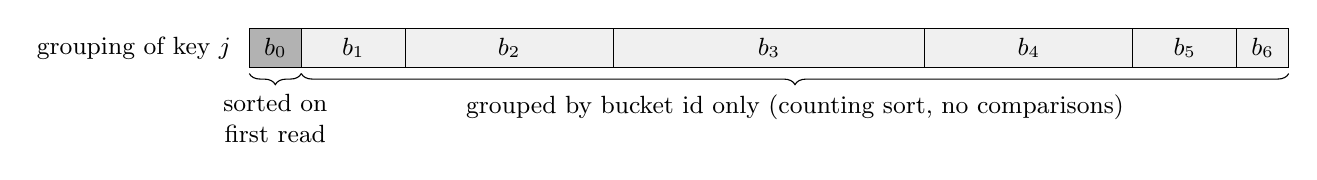
\begin{tikzpicture}[x=0.11cm, y=0.5cm, every node/.style={font=\small}]
  % bucket boxes, widths proportional to the geometric plan
  \def\ys{0}
  \foreach \x/\w/\l in {0/6/0, 6/12/1, 18/24/2, 42/36/3, 78/24/4, 102/12/5, 114/6/6} {
    \draw[fill=black!6] (\x,0) rectangle ++(\w,1);
    \node at (\x+\w/2,0.5) {$b_{\l}$};
  }
  \draw[fill=black!30] (0,0) rectangle ++(6,1);
  \node at (3,0.5) {$b_0$};
  \draw[decorate,decoration={brace,amplitude=4pt,mirror}] (0,-0.15) -- (6,-0.15)
    node[midway,below=4pt,align=center] {sorted on\\first read};
  \draw[decorate,decoration={brace,amplitude=4pt,mirror}] (6,-0.15) -- (120,-0.15)
    node[midway,below=4pt] {grouped by bucket id only (counting sort, no comparisons)};
  \node[anchor=east] at (-1,0.5) {grouping of key $j$};
\end{tikzpicture}
\caption{The grouping of one sort key after a column click: positions are
ordered by stored bucket id; only the first bucket, about one page, is sorted
before the first page is shown. Bucket widths follow the default geometric
plan.}
\label{fig:grouping}
\end{figure}

\section{Analysis}\label{sec:analysis}

\begin{theorem}[Exactness]
For any layout, \textsc{Read}$(i, i+p)$ returns the elements at positions
$i,\dots,i+p-1$ of a stable sort of $S$ by sort key $j$ in the chosen
direction.
\end{theorem}
\begin{proof}
Let $\sigma_0 \prec \dots \prec \sigma_{k-2}$ be the split points. An element
$x$ is in bucket $b$ exactly when $\sigma_{b-1} \preceq x \prec \sigma_b$
(with $\sigma_{-1} = -\infty$, $\sigma_{k-1} = +\infty$); for keyed keys with a
stored split element, the comparison against $\sigma_b$ uses the normalized
key and then the tie-breaker, which is the key's order. Hence for $x$ in bucket
$a$ and $y$ in bucket $b$ with $a < b$ we have $x \prec y$, and elements that
compare equal are in the same bucket. The grouping lists the buckets in
increasing id and, by the counting sort, the elements of each bucket in
insertion order. Sorting a bucket with a stable sort therefore yields exactly
the corresponding segment of the stable sort of $S$, and the concatenation of
all segments is the stable sort itself. A read sorts every bucket it touches
before copying, so the positions it returns are final. Descending order
reverses the bucket order and, within a bucket, the order of runs of equal
elements while keeping each run in insertion order, which is the stable
descending sort; with groups the same argument applies within each group.
\end{proof}

The layout thus affects only the cost of reads. A poor sample, a skewed
distribution or a plan that does not fit the data can make the first bucket
large, which slows the first read, but cannot change the order.

\paragraph{Inconsistent comparators.} The theorem assumes a total preorder.
Real comparators are not always one (Section~\ref{sec:defects}); with a
cyclic comparator no order is correct, and \texttt{std::sort} has undefined
behaviour. Bucketization only partitions elements and merge-sorts buckets, and
neither step can lose or duplicate an element whatever the comparator returns.
With an inconsistent comparator, every element is still returned exactly once.

\paragraph{Costs.} Table~\ref{tab:costs} summarizes the costs. For comparator-only
keys, loading costs $n \lceil \log_2 k \rceil$ comparator calls per key, against
about $n \log_2 n$ for one full sort: with $k = 64$ and $n = 10^5$, about a third.
A switch costs $n + k$ memory operations and no comparisons; on $10^6$
elements this pass, not the sorting of the first bucket, dominates the
switch time.

\begin{table}[t]
\centering
\caption{Costs for $n$ elements, $k$ buckets, $m$ sort keys and page size $p$.}
\label{tab:costs}
\begin{tabular}{ll}
\toprule
Operation & Cost\\
\midrule
add one element & $O(m \log k)$; comparator-only keys: $\lceil\log_2 k\rceil$ comparator calls\\
layout estimation & sorting a sample of $s \le 2048$ elements, per key\\
\textsc{SortBy} & $O(n + k)$, no comparisons; $O(1)$ when the grouping is cached\\
first page & sorting the bucket(s) that cover it: $O(b \log b)$, $b \approx \max(p, n/s)$\\
memory & 2\,B bucket id $+$ 8\,B normalized key $+$ 4\,B grouping per element and key\\
\bottomrule
\end{tabular}
\end{table}

\paragraph{The size of the first bucket.} Split positions are computed in
the sample, so a split cannot be placed closer than one sample element to the
start: the first bucket holds at least about $n/s$ elements. With $s=2048$ this
is below one page up to about $130{,}000$ elements. Beyond that the first read
sorts about $n/s$ elements, still a small fraction of $n$: on the
1{,}000{,}000-entry camera roll the first page cost
\bz{dol@fpc@1000000} element sorts, depending on the column, against
\bz{dol@fpc@100000} at 100{,}000 entries. A larger sample, or a second
sampling round inside the first bucket, would lower this bound; we have not
needed either.

\section{Implementation}\label{sec:impl}

The reference implementation is a header-only C++17 library of about 1{,}800
lines (\texttt{speedup::bucketization}). Its interface,
\texttt{BucketedList<T>}, is implemented by \texttt{BucketIndex<T>}:

\begin{verbatim}
BucketIndex<File> files(BucketPlan::defaults().with_page_size(rows));
files.add_sort_key(SortKey<File>::of("name", &File::name));
files.add_sort_key(SortKey<File>::of("modified", &File::modified)
                       .with_groups(2, [](const File& f) { return f.is_dir ? 0 : 1; }));
files.add_all(list_directory());          // pre-sort: every key, once
files.sort_by("modified", Direction::descending);
for (const File& f : files.range(first, first + rows)) draw(f);
\end{verbatim}

A pure-Java port follows the same interface. A cross-language specification
fixes the normalized-key encodings, the sampling (a SplitMix64
generator~\cite{steele2014splitmix} with a fixed seed), the split rule and the
bucket ids, so that conforming ports produce identical bucket ids for the same
data; both implementations check the same golden values in their test suites.
The C++ unit tests also count comparator calls: on 100{,}000 elements with a
comparator-only key, the first page after a switch costs 569 comparisons,
against about 1.66 million for a full sort.

The index is not thread-safe, even for concurrent reads, because reads sort
lazily; a view model guards it with its existing lock.

\section{Evaluation}\label{sec:eval}

\subsection{Setup}

\paragraph{Machines.} The reference runs used a 4-vCPU Intel Xeon at 2.1\,GHz
cloud container with Ubuntu 24.04, GCC 13.3 (\texttt{-O3}), Qt 6.4.2, ICU 74.2
and GLib 2.80. The portable benchmarks were repeated on a desktop AMD Ryzen 5
2600X (Zen+, 6 cores, 3.6\,GHz base) with 16\,GB of DDR4-2133 under Windows~10,
with MinGW-w64 GCC 13.2 (\texttt{-O3}). Every number is the median of five runs
(one run for the 1{,}000{,}000-entry dataset in the file-manager stacks), on one
thread unless stated otherwise.

\paragraph{Baselines.} Each project is measured on its own code path for a
column click, extracted from its source at a recorded commit and run on the
same data structures it uses: Dolphin's \texttt{KFileItemModel} comparison
(\texttt{QCollator} on ICU, natural ordering, folders first) with its parallel
merge sort and the bookkeeping after it; GLib collation keys with
\texttt{g\_sequence\_sort} for Thunar, Nemo and Caja and GTK~4's sort model for
Nautilus; the Qt sort paths of PCManFM-Qt, the KDE file dialogs and Krusader;
nnn's C comparator; the Godot editor's FileSystem dock; and yazi and lf in their
native languages (Rust and Go), each through a small harness around the
project's sort function. Bucketization uses the same comparison as the
project's tie-breaker, so its order is the project's order by construction,
and every result is checked element by element against the project's own
output. We also compare with \texttt{std::partial\_sort} of the first page,
the obvious ``sort only what is visible'' alternative.

\paragraph{What is measured.} \emph{Re-sort} is the project's time for a
column click. \emph{Switch} is Bucketization's \textsc{SortBy} plus the first
page (64 rows) without a cached grouping, i.e.\ the first time the column is
used after loading. \emph{Pre-sort} is the one-time cost of computing every
element's key and bucket for one column; it can run while the folder is being
listed, or on the first click.

\paragraph{Data.} Real directory listings: \texttt{/usr/bin} (1{,}172
entries), \texttt{/usr/lib/x86\_64-linux-gnu} (1{,}533), the top level of a web
application's \texttt{node\_modules} (395) and the same tree flattened
(36{,}069), all of \texttt{/usr} flattened (97{,}974), and the Linux kernel
source tree (97{,}005, all timestamps equal). Two synthetic camera rolls
(100{,}000 and 1{,}000{,}000 \texttt{IMG\_\ldots} names) and a 20{,}000-name
multilingual set used for correctness checks complete the data.

\subsection{Synthetic workload}

Table~\ref{tab:synthetic} shows the micro-benchmark: one million synthetic
files (a third camera names with long shared prefixes, a third numbered
documents, a third random words; log-normal sizes; random timestamps), four
columns, compared with one \texttt{std::sort} of the column. Showing the first
page after a switch is two to three orders of magnitude faster than a full sort,
a cached switch costs microseconds, and pre-sorting all four columns costs
less than one full sort of any of them. Sorting everything after the switch
costs about a third of a full sort for the numeric columns, whose buckets are
already in order relative to each other. For names it is not a saving: on the
Xeon it took \bz{syn@linux@1000000@name@switch_sort_all_ms}\,ms against
\bz{syn@linux@1000000@name@std_sort_ms}\,ms for \texttt{std::sort}, and on the
Ryzen \bz{syn@windows@1000000@name@switch_sort_all_ms}\,ms against
\bz{syn@windows@1000000@name@std_sort_ms}\,ms. Camera names share long prefixes,
so their normalized keys collide and most comparisons inside the buckets fall
through to the full string comparison, in a stable merge sort. Sorting
everything is not what Bucketization is for, but a view that needs the full
order of a name column at once gains nothing from it.

\begin{table}[t]
\centering
\caption{Synthetic workload, $n=10^6$, milliseconds. Pre-sort registers all
four keys and assigns every element; it is paid once per load. Speed-up is
\texttt{std::sort} over switch $+$ first page.}
\label{tab:synthetic}
\resizebox{\linewidth}{!}{\begin{tabular}{llrrrrrr}
\toprule
Machine & Key & \texttt{std::sort} & Pre-sort & Switch + page & Speed-up & Cached switch & Switch + sort all\\
\midrule
Xeon (Linux) & name & 1{,}052 & 135 & 2.1 & 501$\times$ & 0.0045 & 781\\
 & size & 416 & 130 & 1.8 & 235$\times$ & 0.0049 & 145\\
 & modified & 448 & 137 & 2.1 & 212$\times$ & 0.0048 & 151\\
 & accessed & 433 & 119 & 1.8 & 238$\times$ & 0.0050 & 131\\
\midrule
Ryzen (Windows) & name & 1{,}088 & 152 & 4.5 & 243$\times$ & 0.0038 & 1{,}214\\
 & size & 363 & 138 & 4.3 & 85$\times$ & 0.0048 & 135\\
 & modified & 419 & 137 & 4.0 & 104$\times$ & 0.0050 & 147\\
 & accessed & 358 & 139 & 4.5 & 79$\times$ & 0.0047 & 128\\
\bottomrule
\end{tabular}
}
\end{table}

\subsection{Real file managers}

Table~\ref{tab:projects} summarizes the twelve projects on the large real
listings and the 100{,}000-photo camera roll (four datasets, three columns, two
directions). In every project and every case, the visible rows are final within
\bz{sum@linux@all@switch}\,ms after the click, against
\bz{sum@linux@all@resort}\,ms for the project's own re-sort. The largest gains
are where comparisons are expensive: the Qt-based projects compare names with
\texttt{QCollator} on every comparison, and lf normalizes both names on every
comparison. The smallest are where the project already sorts fast: yazi's Rust
comparator allocates nothing, and the GNOME family compares precomputed
collation keys with \texttt{strcmp}.

\begin{table}[t]
\centering
\caption{Column clicks on the large listings (36{,}069--100{,}000 entries), Xeon
reference machine, milliseconds; ranges over datasets, columns and directions.
\emph{First click slower} counts cases where pre-sort $+$ switch exceeded the
project's re-sort. \emph{Valid orders} counts every dataset, column and
direction, including the small folders; for Dolphin it includes the cases where
Dolphin's own comparator has cycles and no exact order exists
(Section~\ref{sec:defects}).}
\label{tab:projects}
\resizebox{\linewidth}{!}{\begin{tabular}{lrrrrrr}
\toprule
Project & Re-sort today (ms) & Switch + page (ms) & Speed-up & Pre-sort, once (ms) & First click slower & Valid orders\\
\midrule
Dolphin & 59--713 & 0.080--0.72 & 178--3{,}842$\times$ & 2.1--73 & 0/24 & 54/54\\
Thunar & 38--333 & 0.047--0.30 & 218--1{,}552$\times$ & 2.8--10 & 0/24 & 42/42\\
Nemo & 36--382 & 0.057--0.22 & 380--2{,}206$\times$ & 2.6--11 & 0/24 & 42/42\\
Caja & 45--389 & 0.048--0.24 & 312--1{,}953$\times$ & 2.5--10 & 0/24 & 42/42\\
Nautilus & 63--480 & 0.052--0.26 & 729--2{,}921$\times$ & 2.6--12 & 0/24 & 42/42\\
PCManFM-Qt & 48--1{,}499 & 0.092--2.0 & 322--7{,}640$\times$ & 2.6--206 & 0/24 & 42/42\\
KIO dialogs & 84--1{,}384 & 0.079--1.2 & 356--6{,}647$\times$ & 2.0--159 & 0/24 & 42/42\\
Krusader & 115--801 & 0.056--0.54 & 587--4{,}207$\times$ & 1.9--68 & 0/24 & 42/42\\
nnn & 7.7--290 & 0.072--0.28 & 72--1{,}379$\times$ & 1.9--106 & 0/24 & 42/42\\
yazi (native Rust) & 6.3--63 & 0.060--0.33 & 37--425$\times$ & 1.5--12 & 0/24 & 42/42\\
lf (native Go) & 8.0--3{,}050 & 0.057--1.0 & 8.3--12{,}108$\times$ & 1.3--184 & 0/24 & 42/42\\
Godot & 4.3--1{,}165 & 0.089--3.0 & 13--871$\times$ & 1.2--1{,}261 & 6/24 & 36/36\\
\bottomrule
\end{tabular}
}
\end{table}

\paragraph{Against partial sorting.} \texttt{std::partial\_sort} of the first
page with Dolphin's comparison is the strongest simple alternative. On the real
listings it is a median \bz{dol@partial@median}$\times$ slower than a
Bucketization switch (\bz{dol@partial@range}$\times$), and it repeats its work
on every click. Its worst case is a column of equal keys: on the kernel tree
sorted by date, where all timestamps are equal, every comparison falls through
to Dolphin's name comparison and the partial sort takes
\bz{dol@linux-tree@modified@desc@partial}\,ms, against
\bz{dol@linux-tree@modified@desc@switch}\,ms for Bucketization, whose layout
splits the run of equal keys with the tie-breaker.

\paragraph{Opening a folder.} Dolphin sorts all entries before showing the
first row of a folder. Bucketization sorts the visible page after pre-sorting
the visible column: on the three large real listings \bz{dol@open@visible}\,ms
against \bz{dol@open@dolphin}\,ms (\bz{dol@open@speedup}$\times$), and
\bz{dol@open@all}\,ms if all three columns are pre-sorted eagerly
(\bz{dol@open@speedupall}$\times$). Opening therefore becomes faster too,
provided the other columns are pre-sorted lazily, on first use, or in the
background.

\paragraph{Comparator-only keys.} Without a normalized key (Dolphin's
comparison only), switching is as fast as in keyed mode, because a switch
compares nothing either way, but the pre-sort costs
\bz{dol@cmp@presortratio}$\times$ the keyed pre-sort on the large real
listings: every assignment calls the comparator $\lceil\log_2 k\rceil$ times,
while a keyed assignment mostly compares integers.

\subsection{Where it does not help}

\paragraph{Small folders.} Under about 2{,}000 entries every project re-sorts
in a few milliseconds, below one 60\,Hz frame (16.7\,ms). The gain is real but
invisible. Pre-sorting all three columns of the 395-entry folder eagerly is the
one case where Bucketization measured slower than Dolphin (1.39 against
1.03\,ms). An integration should keep the existing sort for small collections
and pre-sort columns on first use.

\paragraph{The first click.} The pre-sort is the price of the first click on a
column, a median of \bz{sum@linux@all@presortmedian}\,ms on the large listings.
It rises to about 200\,ms where the 64-bit key cannot tell the elements apart
and the project's comparator has to break the ties: camera names under ICU
collation keys, identical timestamps tie-broken by name through
\texttt{QCollator}, and nnn's names, whose key needs \texttt{strxfrm} per file.
It stays below one full re-sort of the same folder in every file manager.
The exception is Godot's FileSystem dock, whose own sort is fast for some
columns: there the first click (pre-sort $+$ switch) was slower than Godot's
re-sort in \bz{sum@linux@godot@slower} of 24 large cases; later clicks are not.

\subsection{Second machine}\label{sec:windows}

\IfFileExists{generated/table_projects_windows.tex}{%
Table~\ref{tab:windows} repeats the projects that build without Linux desktop
libraries on the Ryzen desktop under Windows: nnn, the C++ port of lf, Godot,
and yazi natively in Rust (lf's Go program needs a newer Go than was
installed). Table~\ref{tab:synthetic} includes the synthetic workload on that
machine. The conclusions carry over. The switch takes
\bz{sum@windows@all@switch}\,ms, against \bz{sum@windows@all@resort}\,ms for the
projects' own re-sorts (median speed-up \bz{sum@windows@all@speedupmedian}$\times$).
nnn's own re-sort is much slower on Windows than on Linux; it compares names
with the C library's \texttt{strcoll}, whose cost differs between the two
runtimes. Godot's first click was slower than its own re-sort in
\bz{sum@windows@godot@slower} of 24 large cases, against
\bz{sum@linux@godot@slower} on Linux. The switch
itself is about twice as slow as on the Xeon (Table~\ref{tab:synthetic}). It is
mostly a pass over memory, and the desktop's memory ran at only 2133\,MT/s, which
is a likely cause.

\paragraph{One column could not be reproduced on Windows.} nnn's name column
failed the order check in \bz{sum@windows@nnn@invalid} of 42 cases on Windows,
and in none on Linux. Bucketization's key for it is the first eight bytes of
\texttt{strxfrm} output, which the C standard requires to order strings like
\texttt{strcoll}. The Windows C runtime (UCRT, used by both MSVC and MinGW-w64)
breaks that rule in its English locales: \texttt{strcoll} places
\texttt{x-terminal-emulator} before \texttt{xterm}, and \texttt{strcmp} on the
\texttt{strxfrm} output after it. Our checker
(\texttt{speedup\_check\_strxfrm}) finds 245 of 686{,}206 pairs of names in
\texttt{/usr/bin} and 305 of 1{,}174{,}278 in \texttt{/usr/lib} ordered
differently in \texttt{en\_US.UTF-8}, and none in the \texttt{C} locale. A key built from \texttt{strxfrm} is therefore not order-preserving on Windows
and cannot reproduce \texttt{strcoll}'s order there; a comparator-only sort key,
which calls \texttt{strcoll} itself, can. Table~\ref{tab:windows} reports nnn's timings for
the orders that passed the check only.

\begin{table}[t]
\centering
\caption{The portable projects on the Ryzen 5 2600X under Windows~10 (MinGW-w64
GCC 13.2), milliseconds, same datasets and method as Table~\ref{tab:projects}.
Timings cover only the orders that passed the order check; for nnn, its name
column failed it on Windows (Section~\ref{sec:windows}).}
\label{tab:windows}
\resizebox{\linewidth}{!}{\begin{tabular}{lrrrrrr}
\toprule
Project & Re-sort today (ms) & Switch + page (ms) & Speed-up & Pre-sort, once (ms) & First click slower & Valid orders\\
\midrule
nnn & 36--2{,}257 & 0.14--0.69 & 145--4{,}639$\times$ & 2.6--285 & 0/18 & 32/42\\
yazi (native Rust) & 7.7--67 & 0.089--0.43 & 40--286$\times$ & 1.3--16 & 0/24 & 42/42\\
lf (C++ port) & 4.0--1{,}904 & 0.080--1.2 & 8.8--6{,}503$\times$ & 1.1--336 & 0/24 & 42/42\\
Godot & 3.6--2{,}391 & 0.13--6.4 & 5.2--879$\times$ & 1.6--2{,}510 & 8/24 & 36/36\\
\bottomrule
\end{tabular}
}
\end{table}
}{The Windows re-run is pending.}

\section{Comparator defects found}\label{sec:defects}

Checking Bucketization's output against each project's own order requires that
order to be well defined. Three projects' comparators turned out not to be:

\paragraph{Dolphin's natural comparison has cycles.} It reads a two-part
number such as \texttt{6.10} as a decimal ($6.10 < 6.9$) but compares two-part
with three-part numbers part by part ($6.9.1 < 6.10$). Ordinary file names
therefore form cycles:
\texttt{kernel-6.10.tar.xz} $<$ \texttt{kernel-6.9.tar.xz} $<$
\texttt{kernel-6.9.1.tar.xz} $<$ \texttt{kernel-6.10.tar.xz}.
No sort can produce a consistent order for such names; the order Dolphin shows
depends on the order in which the folder was listed. On the multilingual set,
even \texttt{std::stable\_sort} with Dolphin's comparison disagrees with
Dolphin's own merge sort in 32 of 20{,}000 positions.

\paragraph{Krusader's descending comparator is not a strict weak ordering.}
It is defined as the negation of the ascending one, so for two items that
compare equal (\texttt{README} and \texttt{readme} under the default
case-insensitive setting) it returns true in both directions, and it returns
true for an item compared with itself. It is passed to \texttt{std::stable\_sort}
and \texttt{std::lower\_bound}, whose behaviour is then undefined; libstdc++'s
debug mode reports the violation.

\paragraph{lf normalizes names on every comparison.} Its natural ordering
removes diacritics and lowers the case of both names inside the comparator, so
each sort allocates and normalizes $O(n\log n)$ strings. Normalizing once per
file makes name sorting 4--8 times faster on large folders. This is a
performance issue, not a correctness one.

All three were reported to the projects in October 2026, independently of
Bucketization. Because comparators like these exist, Bucketization sorts buckets
only with merge sorts, which tolerate inconsistent comparators
(Section~\ref{sec:analysis}).

\section{Related work}\label{sec:related}

\paragraph{Distribution sorting.} Assigning elements to buckets delimited by
sampled splitters is samplesort~\cite{frazer1970samplesort}; super scalar
samplesort~\cite{sanders2004superscalar} and its in-place parallel
successor~\cite{axtmann2017ips4o} make the assignment branch-free over an
implicit search tree of splitters. Bucketization uses the same assignment, but
stops after it, keeps the bucket ids of every key, and sorts buckets only on
demand. Its buckets have planned, unequal sizes, small at both ends of the
order, while samplesort aims for equal buckets.

\paragraph{Partial and incremental sorting.} Partial
quicksort~\cite{martinez2004partial} produces the $p$ smallest elements in
order in $O(n + p\log p)$ expected time, and incremental
sorting~\cite{paredes2006incremental} produces the elements in order on demand.
Both compare all $n$ elements per query and keep no state across different
sort keys; Bucketization performs these comparisons at load time, once per key,
and a switch compares nothing.

\paragraph{Adaptive indexing.} Database cracking~\cite{idreos2007cracking}
reorganizes a column incrementally as a side effect of the range queries that
touch it, so that the work follows the workload. Lazy bucket sorting follows
the same principle, with the view's scroll position as the workload.

\paragraph{Normalized and abbreviated keys.} Database systems compare
order-preserving binary prefixes of keys and fall back to full comparisons only
on ties~\cite{graefe2006sorting}; PostgreSQL's abbreviated keys apply this to
collated text~\cite{postgres95}. Bucketization's normalized keys are such
prefixes, used both for bucket assignment and inside bucket sorts.

\paragraph{Per-column sorted indexes.} A view could also sort every column
fully when the data is loaded and keep the permutations, making every later
switch $O(1)$. That costs $m$ full sorts at load ($\Theta(mn\log n)$
comparisons) and $O(\log n)$ comparator calls per update and key; Bucketization
needs $mn\lceil\log_2 k\rceil$ comparisons at load and sorts only what is shown,
which is what makes opening a folder faster rather than slower.

\section{Limitations}\label{sec:limits}

The file-manager measurements cover the sorting stage only, not listing the
directory, creating items or drawing the view, and the extracted sort paths
were run outside the applications. The reference results come from one cloud
container; the second machine covers only the projects that build without Linux
desktop libraries. Dolphin's name sort uses four threads in our measurements
while Bucketization uses one, which favours Dolphin. The camera rolls and the
multilingual set are synthetic. Bucketization costs 14 bytes per element and
sort key, plus one pointer or handle per element. Finally, the design targets
views that are read from the start or the end; a view that jumps to the middle
of a large collection sorts one of the large middle buckets on the first read.

\section{Conclusion}

Re-sorting a multi-column view on every click spends almost all of its time on
elements the user cannot see. Bucketization assigns every element to a
bucket of every column once, when it is loaded, and turns the click into a
counting pass and the sorting of one page-sized bucket, while keeping the order
exact. In the sort code of twelve real projects this moved column switches on
large folders from tens or hundreds of milliseconds, sometimes seconds, to
well under a frame. The C++ and Java implementations, all benchmarks, the
captured listings and the scripts that produced every number in this paper are
open source.

\section*{Availability}

Source code, data and scripts: \url{https://github.com/attilatorda/SpeedUp}
(AGPL-3.0, with an additional permission for the file managers named in the
repository). The numbers in this paper are generated from the result files in
\nolinkurl{benchmarks/outputs/} by
\nolinkurl{benchmarks/scripts/bucketization_paper_numbers.py}.

\bibliographystyle{plainnat}
\bibliography{refs}

\end{document}
